%
\vspace{5pt}
\subsubsection{Number of hidden states}
\vspace{5pt}
\begin{figure}[h!]
 \centering
 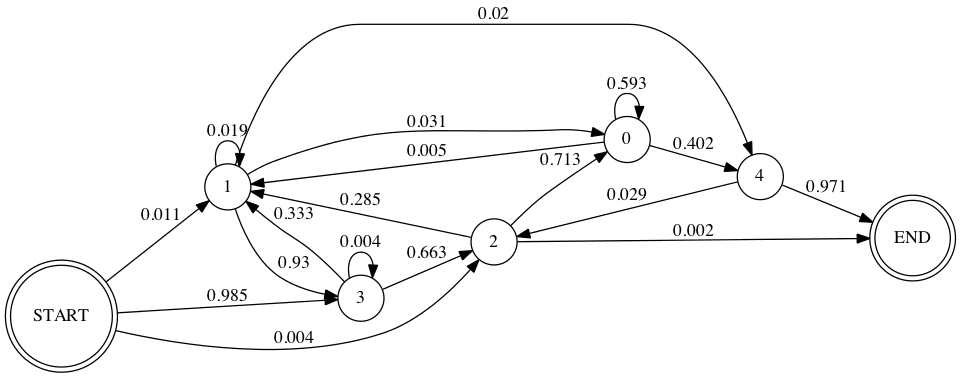
\includegraphics[width=1\textwidth]{./figure/HiddenMarkov5.png}
 \caption{trnasition graphic model with 5 hidden state: In this figure, we ignore transition probability lower than $10 ^{-4}$ and we can see that some of the transition between states are ignorable, which is a indication that hidden states do have their own iterpretations}
 \end{figure}
\paragraph{} First, as we increase the number of hidden states, the quality of the generated sentences is increasing. We interpret this phenomenon as such: when the number of hidden states is small, some very different word have to be put into the same state. When generating sequences, not all word pairs under consecutive hidden states are meaningful(actually only a small number of pairs are). If we increase the number of hidden states to be almost equal to the number of words in the corpus, then usual word pairs are easily captured. Another benefit of increasing number of hidden states is that the sentence length is tending to have less variation. We randomly generate 1000 sentences when the number of hidden states equals 5, 100 and 1000 and plot the generated sentence length distribution. We find that as the number hidden states increases, the sentence length is more centered around 8-9, which is the typical length of a line in a sonnet.
%\begin{figure}[ht]
%\centering
%\begin{minipage}[b]{0.45\linewidth}
%	\centering
%  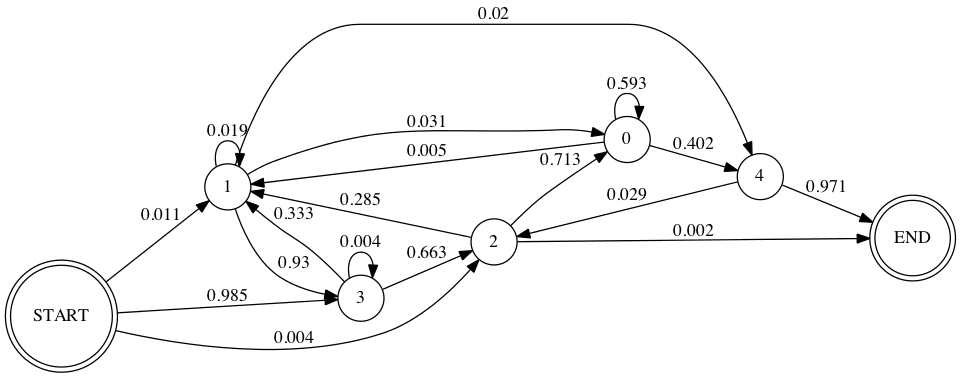
\includegraphics[width=0.6\linewidth]{./figure/HiddenMarkov5.png}
%  \caption{Happy Smiley}
%  \label{fig:minipage1}
%\end{minipage}
%\quad
%\begin{minipage}[b]{0.45\linewidth}
%	\centering
%  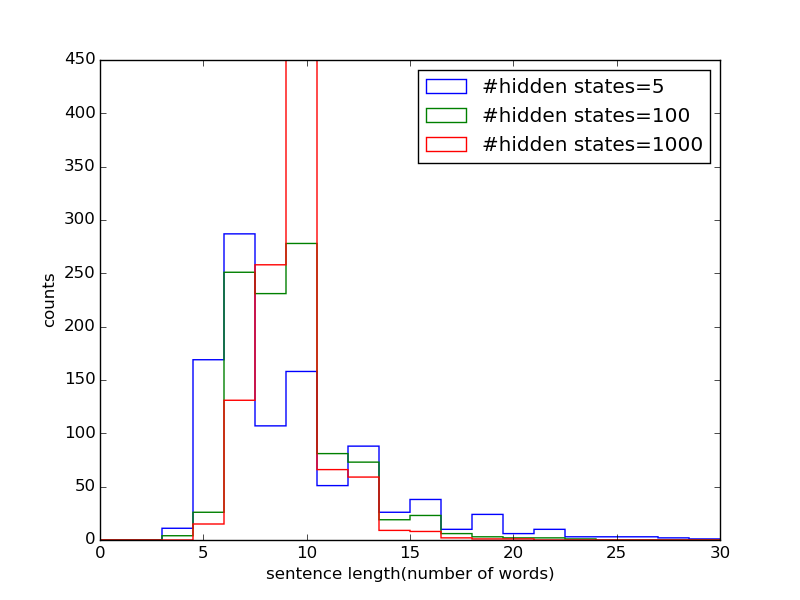
\includegraphics[width=0.6\linewidth]{./figure/hiddenstate_len_distri.png}
%  \caption{Sad Smiley}
%  \label{fig:minipage2}
%\end{minipage}
%\end{figure}

 \begin{figure}[h!]
 \centering
 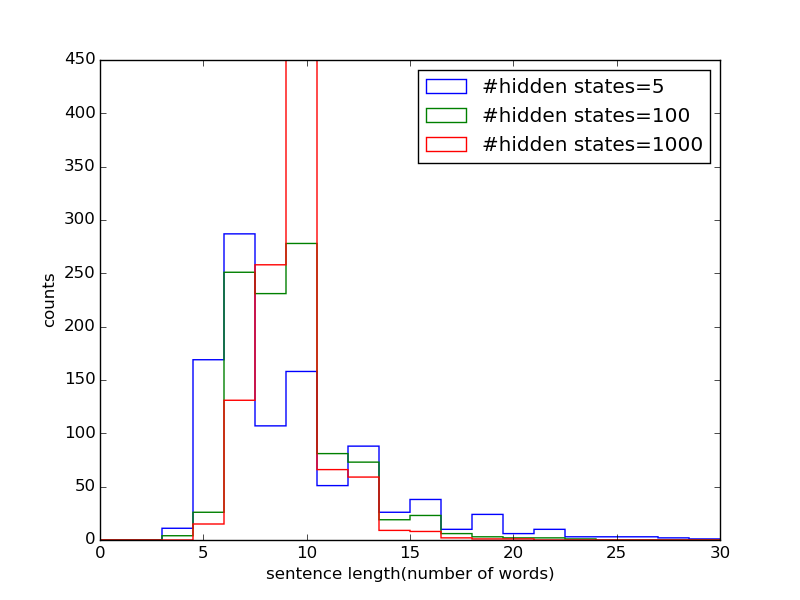
\includegraphics[width=0.5\textwidth]{./figure/hiddenstate_len_distri.png}
 \caption{Sentence length distribution with different number of hidden states. When number of hidden states=1000, the length of the sentences are centered arount 8-9.}
 \end{figure}
\vspace{5pt}
\subsection{Interpreting the hidden states}
\vspace{5pt}

\paragraph{} Here we also present our findings about the interpretations of the hidden states.
The hidden states should bear some meanings in a sense that words likely to be emitted from the same hidden states should more or less share some common features. We find that the words pertaining to different hidden state may have difference in their part of speech tag, syllables and positions in a sentence.

For simplicity, in the following discussion we are always using 5 hidden states example.  We plot the transition diagram of the 5 hidden states. From that we can see there is a close connection between hidden states and the position in a sentence.
For each sentence in the training corpus, we use Viterbi algorithm to find the most likely corresponding hidden state sequences.We count how many times a certain state appears in a certain position of a sentence.  We plot out the distribution of the occurring position of the 5 hidden states in those maximum likelihood sequences. 
It is clear that each of the 5 hidden states have peaks in different positions of a sentence. State 2 is most likely to be the starting word of a sentence while state 4 end of a sentence.
 \begin{wrapfigure}[20]{l}{0.5\textwidth}
 %\begin{center}
 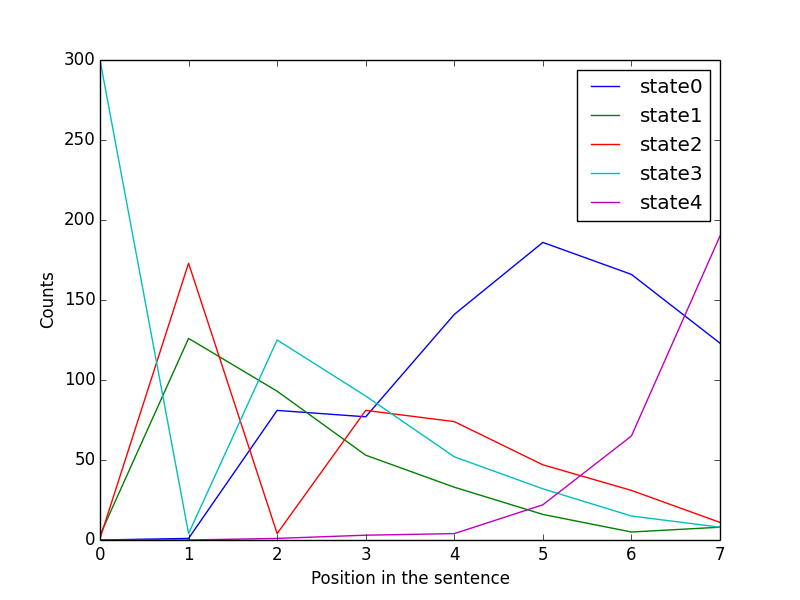
\includegraphics[width=0.5\textwidth]{./figure/hiddenstates_position_in_the_sentence.png}
 \caption{The distribution of different hidden states showing up at different positions in a sentence. Here we assume that a sentence is made of 8 words. If the actual length is greater than 8, then the later positions are also categorized as position 7.\label{fig:position}}
 %\end{center}
\end{wrapfigure}
\section*{}
\vspace{10pt}
\paragraph{}
Words pertaining to the 5 hidden states also have different distribution in their corresponding part of speech tags.  For each sentence in the corpus, we use the part of speech tags marking tools provided by NLTK package to see the part of speech tag each hidden state is corresponding to and then make a histogram of how many times a hidden states appears in a sentence as a noun, verb, adj, adv,. We find that state 1 is most likely to appear as a noun while state 2 is more likely to appear as verb. Conjunction words like \textbf{'and'},\textbf{'or'} are more likely to be under state 2 and 3 while state 4, usually at the end of a sentence, is limited to noun and verb. \ref{fig:position} illusstrates the relationship between hidden states and positions in a sentence.
\\
\\
 \begin{figure}[h]
 \centering
 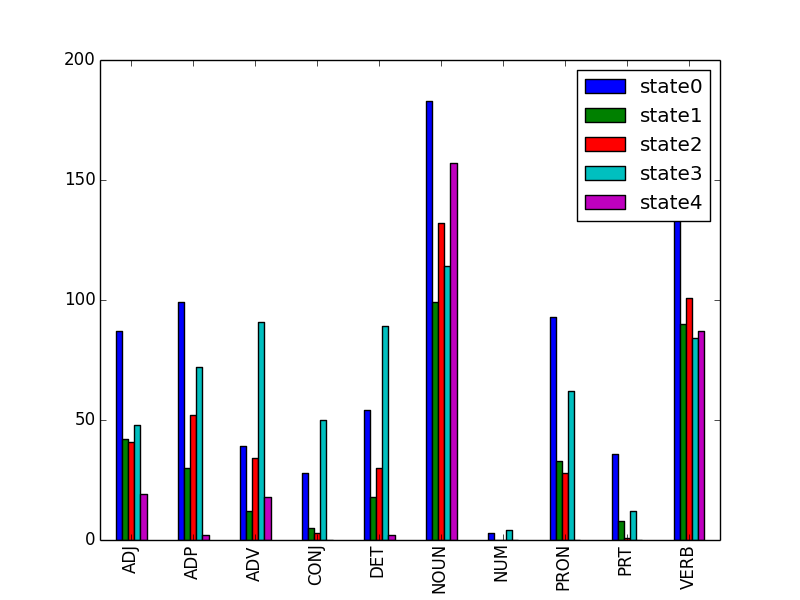
\includegraphics[width=0.5\textwidth]{./figure/hiddenstate_partofspeechtag.png}
 \caption{Statistics of corresponding part of speech tag for each state in the maximum likelyhood sequence given by viterbi algorithm}
 \end{figure}
\paragraph{}
%\vspace{35pt}
\section*{}
The number of syllables in each state is not so different. We choose the most probable 200 word that is emitted by each of the 5 states and count their number of syllables. The emitting probability has been normalized by word frequency. We didn’t find significant differences between each state. 


\paragraph{}
To make a conclusion, the five states has clear meaning representing the position in a sentence. It also has some relationship to the part of speech tags. But the two effects are not independent. It might be that a certain state have to be the first state in a sentence so that it prefers some part of speech tags rather than others. In this study, the hidden state doesn't seem to bear sentimental meanings because the corpus is so small and most words appear only once. So there is no way to tell their sentimental polarity. If we have a larger corpus, by using more hidden states, we could dig out more sentimental meanings. 
%\newline
 \begin{wrapfigure}[16]{r}{0.5\textwidth}
 \centering
 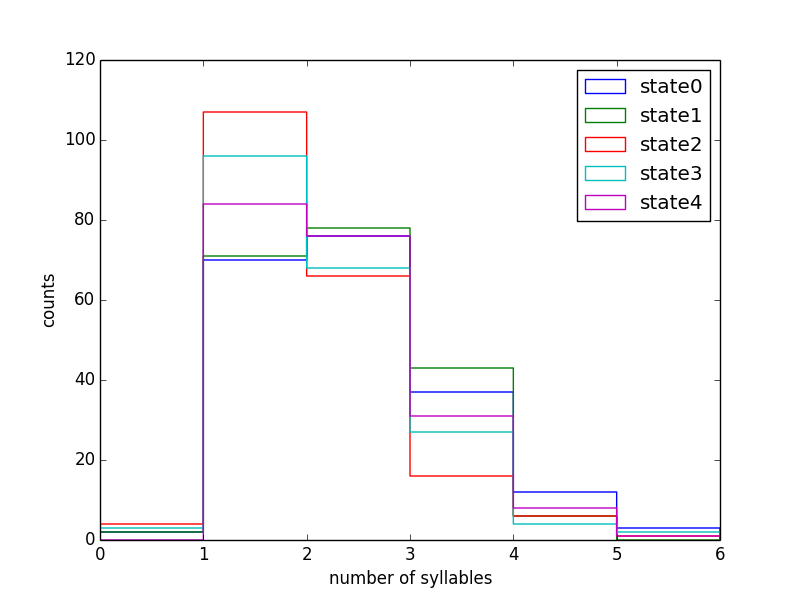
\includegraphics[width=0.5\textwidth]{./figure/numberofsyllablesinstates.png}
 \caption{Number of syllables in the most probable 200 emitting words for each hidden state.}
\end{wrapfigure}
